% ==============================================================
% Modelo para Relatório Parcial de Iniciação Científica da UFES
% Prof. Vítor E. Silva Souza - DI/CT/UFES :: PPGI/CT/UFES
%
% Baseado no modelo fornecido pela PRPPG/UFES:
% https://prppg.ufes.br/programa-institucional-de-ic-piic
%
% This work may be distributed and/or modified under the
% conditions of the LaTeX Project Public License, either version
% 1.3 of this license or (at your option) any later version. The
% latest version of this license is in
% http://www.latex-project.org/lppl.txt.
% ==============================================================
\documentclass[12pt, a4paper]{article}

% Importa pacotes a serem utilizados no documento.
\usepackage{graphicx,color}
\usepackage[dvipsnames]{xcolor,colortbl}
\usepackage[hidelinks]{hyperref}
\usepackage{anysize}
\usepackage{graphicx}
\usepackage{iftex}
\ifPDFTeX
  \usepackage[utf8]{inputenc}
  \usepackage[T1]{fontenc}
\else
  \usepackage{fontspec}
\fi
% babel: texlive-lang-portuguese não instalado; inputenc+fontenc cobrem UTF-8 PT-BR
% \usepackage[brazil]{babel}
\usepackage{fancyhdr}
\usepackage{ifthen}
\usepackage{array}
\usepackage{natbib}
\usepackage{amsmath}
\usepackage{enumerate}
\usepackage{adjustbox}
\usepackage{titlesec}
\ifPDFTeX
  \usepackage{mathptmx}
\fi
\usepackage{booktabs}
\usepackage{float}

% Reduz o espaço entre os itens da bibliografia
\let\oldbibliography\thebibliography
\renewcommand{\thebibliography}[1]{\oldbibliography{#1}
\setlength{\itemsep}{0pt}}

% Configura a fonte do documento.
\ifPDFTeX
  \usepackage{helvet}
  \renewcommand{\familydefault}{\sfdefault}
\else
  \setmainfont{Arial}
  \setsansfont{Arial}
  \renewcommand{\familydefault}{\sfdefault}
\fi

% Configura espaçamento 1,5 entre linhas.
\usepackage{setspace}
\onehalfspacing

% Configura espaçamento entre os parágrafos.
\usepackage{parskip}
\setlength{\parindent}{0pt}
\setlength{\parskip}{6pt}

% Configura tamanho dos títulos.
\titleformat{\section}
  {\normalfont\fontsize{14}{16}\bfseries}{\thesection}{1em}{}[{\titlerule[0.8pt]}]

% Configura o tamanho e alinhamento das legendas.
\usepackage{caption}
\usepackage{subcaption}
\captionsetup{font={footnotesize}, labelsep=endash}
\captionsetup{singlelinecheck=false,justification=raggedright}
\captionsetup[subfigure]{justification=centering, singlelinecheck=true}
\captionsetup[figure]{skip=2pt}
\captionsetup[quadro]{skip=2pt}

% Cria um tipo coluna com alinhamento à esquerda.
\usepackage{tabularx}
\newcolumntype{L}[1]{>{\raggedright\arraybackslash}p{#1}}

% Define os elementos gráfico e quadro.
\usepackage{newfloat}
\renewcommand{\figurename}{Figura}
\renewcommand{\tablename}{Tabela}
\DeclareFloatingEnvironment[name={Gráfico}]{grafico}
\DeclareFloatingEnvironment[name={Quadro}]{quadro}

% Configura listas enumeradas.
\usepackage{enumitem}
\setlist[enumerate]{nosep}

% Permite inclusão de notas, úteis para revisão.
\setlength{\marginparwidth}{2cm}
\usepackage[colorinlistoftodos, textwidth=20mm, textsize=footnotesize]{todonotes}
\newcommand{\aluno}[1]{\todo[author=\textbf{Aluno},color=green!30,caption={},inline]{#1}}
\newcommand{\professor}[1]{\todo[author=\textbf{Professor},color=red!30,caption={},inline]{#1}}

% Permite usar o comando \hl{} para evidenciar texto.
\usepackage{soul}

% Permite colocar espaços no final das macros quando necessário.
\usepackage{xspace}

% Definição de símbolos para o cronograma.
\usepackage{amssymb}
\usepackage{pifont}
\usepackage{tikz}
\newcommand{\totalmente}{\ding{51}\xspace}
\newcommand{\parcialmente}{%
\begin{tikzpicture}[baseline=-0.5ex]
    \draw (0,0) circle (0.8ex);
    \fill (0,0) -- (90:0.8ex) arc (90:270:0.8ex) -- cycle;
\end{tikzpicture}}
\newcommand{\naorealizada}{%
\begin{tikzpicture}[baseline=0ex, line width=0.25ex]
    \draw (0,0) -- (1.2ex,1.2ex);
    \draw (0,1.2ex) -- (1.2ex,0);
\end{tikzpicture}}

% Definição de macros.
\newcommand{\java}{Java\texttrademark\xspace}

% Configuração das margens.
\usepackage[a4paper, left=30mm, top=30mm, right=20mm, bottom=20mm, includehead, headsep=25mm, headheight=35pt]{geometry}
\addtolength{\voffset}{-25mm}
\addtolength{\textheight}{25mm}

% Definição do cabeçalho.
\usepackage{afterpage}
\pagestyle{fancy}
\fancyhf{}
\fancyhead[R]{\fontsize{10}{12}\selectfont\color{Gray} Universidade Federal do Espírito Santo\\ Programa Institucional de Iniciação Científica\\ Relatório Parcial de Pesquisa\\ Ciência da Computação}
\renewcommand{\headrulewidth}{0pt}

% Definição do rodapé.
\fancyfoot[R]{\thepage}
\renewcommand{\footrulewidth}{0pt}

% Início do documento.
\begin{document}

\bgroup
\def\arraystretch{1.1}
\begin{tabularx}{\textwidth}{|>{\columncolor{gray!25}}L{59mm}|L{88mm}|}
\hline
{\bf Edital:} & {\bf Edital PIIC 2025/2026} \\
\hline
{\bf Área do Conhecimento (CNPq):} & {\bf Ciência da Computação} \\
\hline
{\bf Subárea do Conhecimento (CNPq):} & {\bf Metodologia e Técnicas da Computação} \\
\hline
{\bf Título do Projeto:} & {\bf Pesquisa Operacional e Inovação em Logística Regional} \\
\hline
{\bf Título do Subprojeto:} & {\bf Otimização Dinâmica de Rotas para Coleta de Resíduos Sólidos: Adaptação do Algoritmo de Solomon com Integração IoT} \\
\hline
{\bf Orientador(a):} & {\bf Maria Claudia Silva Boeres} \\
\hline
{\bf Estudante:} & {\bf Emilly Lopes Das Neves} \\
\hline
\end{tabularx}
\egroup
\vspace{2mm}

\bgroup
\def\arraystretch{1.1}
\begin{tabularx}{\textwidth}{|>{\columncolor{gray!25}}L{59mm}|L{42mm}|L{42mm}|}
\hline
{\bf Estudante apresenta alguma necessidade de acessibilidade?} & {\vspace{1mm} Sim (\ \ \ )} & {\vspace{1mm} Não (\ X\ )} \\
\hline
{Se sim, informar o recurso ou suporte de acessibilidade que necessita.} & \multicolumn{2}{|l|}{ } \\
\hline
\end{tabularx}
\egroup
\vspace{.5cm}

% ---------------------------------------------------------------
\section{Introdução}
\label{sec-intro}

A gestão de resíduos sólidos urbanos impõe desafios operacionais, econômicos e ambientais aos serviços municipais. Sistemas convencionais de coleta, baseados em rotas fixas e frequências predeterminadas, podem gerar deslocamentos desnecessários e dificultar respostas adequadas a situações de enchimento crítico dos recipientes \citep{pardini2020smart, lozano2018smart}. Nesse contexto, a literatura aponta que a integração entre monitoramento em tempo real e técnicas de otimização pode contribuir para um planejamento de coleta mais eficiente \citep{lozano2018smart, barth2023data}.

O subprojeto de Iniciação Científica, vinculado ao Projeto ``Pesquisa Operacional e Inovação em Logística Regional'', propõe uma solução integrada que combina sensores IoT via LoRaWAN \citep{ramson2021lorawan, de2021plataforma} com heurísticas baseadas no algoritmo de \citet{solomon1987algorithms} para o Problema de Roteamento de Veículos com Janelas Temporais (VRPTW), além do uso de um Digital Twin para apoio à simulação e à visualização das rotas \citep{barth2023data}. A pergunta de pesquisa que orienta o desenvolvimento desse trabalho consiste em verificar de que modo a integração entre monitoramento IoT e heurísticas clássicas para o VRPTW pode tornar o planejamento da coleta mais responsivo e eficiente, preservando a factibilidade temporal das rotas. Este relatório parcial descreve as atividades desenvolvidas no primeiro semestre de trabalho, com ênfase na revisão bibliográfica, na definição da arquitetura do sistema, na implementação dos algoritmos de otimização e no desenvolvimento inicial do ambiente de integração com sensores.


% ---------------------------------------------------------------
\section{Materiais e Métodos}
\label{sec-metodo}

Para a realização desse projeto, foram estudados e implementados para o VRPTW a heurística construtiva de inserção de \citet{solomon1987algorithms}, o VND \citep{hansen2001variable}, o GRASP nas variantes fixa e reativa \citep{feo1995greedy, resende2003greedy, prais2000reactive} e a Busca Tabu \citep{glover1989tabu, glover1990tabu}, que compõem o solver desenvolvido.

Implementado em C++20, o solver é avaliado nas instâncias clássicas de 100 clientes de \citet{solomon1987algorithms}, segundo o critério do 12º Desafio DIMACS para o VRPTW\footnote{Disponível em: \url{http://dimacs.rutgers.edu/programs/challenge/vrp/vrptw/}.}, que minimiza a distância total com uma casa decimal. A formulação clássica de \citet{solomon1987algorithms} emprega duas casas decimais e hierarquia veículos-distância; por isso, ambas as abordagens permanecem implementadas para comparação nas próximas etapas.

As instâncias de 100 clientes de \citet{solomon1987algorithms} distribuem-se nas famílias C, R e RC, correspondentes a distribuições agrupada, aleatória e mista. Cada instância define coordenadas, demanda, janela de tempo, tempo de serviço e um depósito central com frota homogênea de capacidade fixa.

A metodologia incluiu a avaliação de operadores de busca local \citep{toth2002vehicle, potvin1995exchange}, com movimentos intra-rota (Relocate intra, Swap intra, 2-opt intra) e entre rotas (Relocate inter, Swap inter, 2-opt inter, Or-opt e Cross-exchange), seguida da seleção de um subconjunto mais promissor. A comparação entre configurações utilizou testes não paramétricos com controle de múltiplas comparações \citep{demsar2006statistical}, e a calibração do GRASP e da Busca Tabu foi realizada com o pacote \textit{irace} \citep{lopez2016irace}. Toda solução produzida é validada quanto à cobertura de clientes, à capacidade veicular e à viabilidade das janelas de tempo.

Também foi planejada e iniciada a implementação de um ambiente de simulação de sensores IoT, inspirado em \citet{lozano2018smart} e \citet{de2021plataforma}, para avaliar a integração entre monitoramento do enchimento e roteamento. O Quadro~\ref{qdr-sensores} resume seus aspectos funcionais previstos.

\begin{quadro}[H]
    \centering
    \caption{Aspectos funcionais do ambiente de simulação de sensores IoT}
    \label{qdr-sensores}
    \fontsize{10}{12}\selectfont
    \begin{tabular}{|p{64mm}|p{82mm}|}
        \hline
        \rowcolor{gray!25}
        \centering\textbf{Componente} & \centering\textbf{Descrição} \tabularnewline
        \hline
        Modelo de enchimento & Distribuição estatística com variação por período (pico e fora de pico) \\
        \hline
        Tecnologia de comunicação & LoRaWAN (simulada) \\
        \hline
        Critério de acionamento & Nível de enchimento acima de limiar configurável \\
        \hline
        Geração de demanda & Lixeiras ativas convertidas em clientes com janela de tempo \\
        \hline
        Interface com o solver & Envio de eventos ao módulo VRPTW a cada ciclo de monitoramento \\
        \hline
        Linguagem de implementação & Python \\
        \hline
    \end{tabular}
    \vspace{5pt}
    \caption*{Fonte: Produção da própria autora.}
    \caption*{\textit{Descrição do Quadro~\ref{qdr-sensores}:} quadro com seis linhas descrevendo os componentes funcionais do ambiente de simulação, desde o modelo de enchimento com variação temporal até a interface de integração com o solver VRPTW.}
\end{quadro}


% ---------------------------------------------------------------
\section{Resultados e Discussão}
\label{sec-resultados}

Os resultados desta seção foram obtidos sob o critério do 12º Desafio DIMACS para o VRPTW, com Solomon I1 \citep{solomon1987algorithms} como referência inicial. As referências do SINTEF/TOP\footnote{\url{https://www.sintef.no/projectweb/top/vrptw/100-customers/}} foram utilizadas como benchmark complementar para situar os melhores valores conhecidos das instâncias. Na avaliação dos operadores de busca local, movimentos entre rotas mostraram contribuição mais consistente do que ajustes intra-rota.

Na análise de busca local, adotou-se o algoritmo VND (Descida em Vizinhança Variável) \citep{hansen2001variable} para selecionar um conjunto reduzido de vizinhanças que preservasse a qualidade das soluções sem ampliar desnecessariamente a complexidade da busca. O Quadro~\ref{qdr-contrib-vnd} sintetiza a contribuição dos principais grupos de operadores.

\begin{quadro}[H]
    \centering
    \caption{Síntese qualitativa da contribuição dos operadores de busca local no VND}
    \label{qdr-contrib-vnd}
    \fontsize{10}{12}\selectfont
    \begin{tabular}{|p{40mm}|p{55mm}|p{45mm}|}
        \hline
        \rowcolor{gray!25}
        \centering\textbf{Grupo de operadores} & \centering\textbf{Contribuição observada} & \centering\textbf{Papel predominante} \tabularnewline
        \hline
        Movimentos entre rotas \newline {\footnotesize(Relocate inter, 2-opt inter)} & Maior impacto nas melhorias mais relevantes & Redistribuição de clientes e reorganização global das rotas \\
        \hline
        Movimentos intra-rota \newline {\footnotesize(Relocate intra, 2-opt intra)} & Contribuição frequente em ajustes finos & Refinamento local da sequência de atendimento \\
        \hline
        Operadores de troca \newline {\footnotesize(Swap intra, Swap inter)} & Efeito complementar ao longo da busca & Correções pontuais de posicionamento dos clientes \\
        \hline
        Operadores mais complexos \newline {\footnotesize(Or-opt, Cross-exchange)} & Uso mais localizado e menos recorrente & Diversificação do processo de busca \\
        \hline
    \end{tabular}
    \vspace{5pt}
    \caption*{Fonte: Produção da própria autora.}
    \caption*{\textit{Descrição do Quadro~\ref{qdr-contrib-vnd}:} quadro com quatro linhas sintetizando o papel dos principais grupos de operadores de busca local, destacando sua contribuição relativa no refinamento das soluções produzidas pelo VND.}
\end{quadro}

O Quadro~\ref{qdr-comparativo} resume o comparativo global que está em fase de desenvolvimento. Em termos gerais, as meta-heurísticas superam qualitativamente o método construtivo de referência, sobretudo quando equilibram qualidade das soluções e tempo de resposta, em linha com os testes estatísticos aplicados \citep{demsar2006statistical}.

\begin{quadro}[H]
    \centering
    \caption{Síntese qualitativa do comparativo entre os algoritmos implementados}
    \label{qdr-comparativo}
    \fontsize{10}{12}\selectfont
    \begin{tabular}{|p{30mm}|p{60mm}|p{50mm}|}
        \hline
        \rowcolor{gray!25}
        \centering\textbf{Algoritmo} & \centering\textbf{Perfil observado} & \centering\textbf{Potencial de uso} \tabularnewline
        \hline
        \mbox{Solomon I1} \mbox{(referência)} & Construção inicial simples e rápida & Referência para comparação e geração de solução inicial \\
        \hline
        VND & Refinamento local com baixo tempo de resposta & Cenários com maior restrição temporal \\
        \hline
        GRASP fixo & Melhoria consistente com maior esforço computacional & Planejamento com maior margem de processamento \\
        \hline
        GRASP reativo & Boa robustez no refinamento das soluções & Instâncias heterogêneas e ajustes iterativos \\
        \hline
        Busca Tabu & Boa qualidade com resposta mais ágil do que abordagens mais intensivas & Replanejamento mais frequente \\
        \hline
    \end{tabular}
    \vspace{5pt}
    \caption*{Fonte: Produção da própria autora.}
    \caption*{\textit{Descrição do Quadro~\ref{qdr-comparativo}:} quadro com cinco linhas, uma por algoritmo, sintetizando o perfil de desempenho observado e seu potencial de aplicação no contexto do roteamento com janelas de tempo.}
\end{quadro}

Quanto ao módulo de simulação de sensores, a versão inicial confirmou a geração de eventos e a comunicação com os algoritmos. 

A Figura~\ref{fig-rotas} compara, sob o critério DIMACS, as rotas produzidas na instância C102, da família C de Solomon, com 100 clientes agrupados em \textit{clusters}, um depósito central e janelas de tempo. Cada painel informa, no rodapé, o custo total e o número de rotas da solução correspondente. Entre os métodos avaliados, o GRASP reativo apresentou o melhor resultado.

\begin{figure}[h!]
    \centering
    \caption{Comparação de rotas na instância C102}
    \label{fig-rotas}
    \begin{subfigure}[t]{0.32\textwidth}
        \centering
        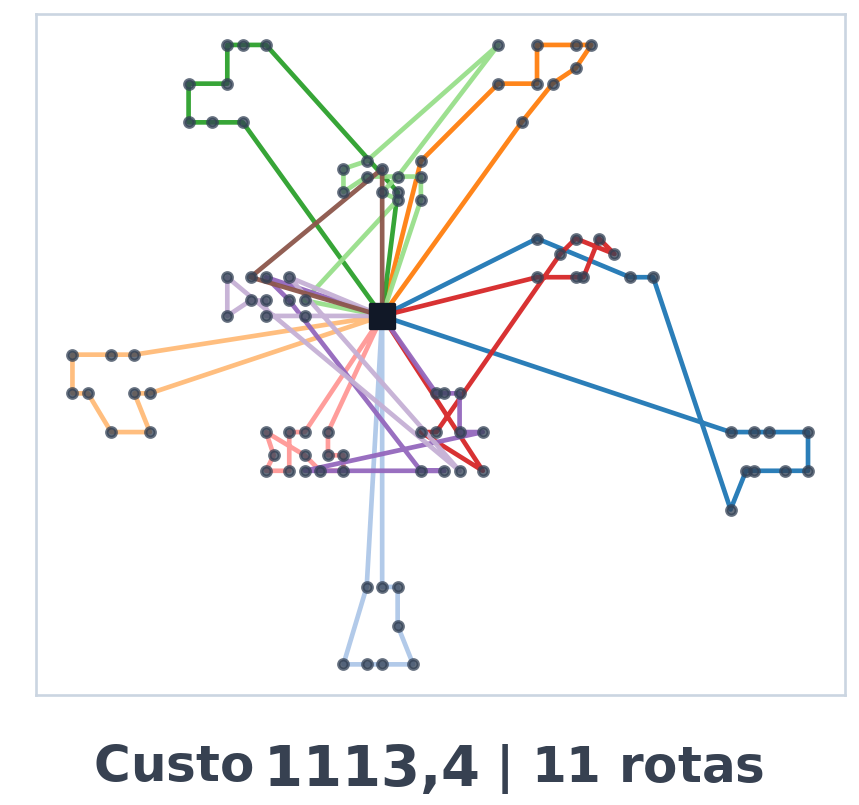
\includegraphics[width=\linewidth]{route_compare_C_panel_1}
        \caption{Solomon I1}
    \end{subfigure}
    \hfill
    \begin{subfigure}[t]{0.32\textwidth}
        \centering
        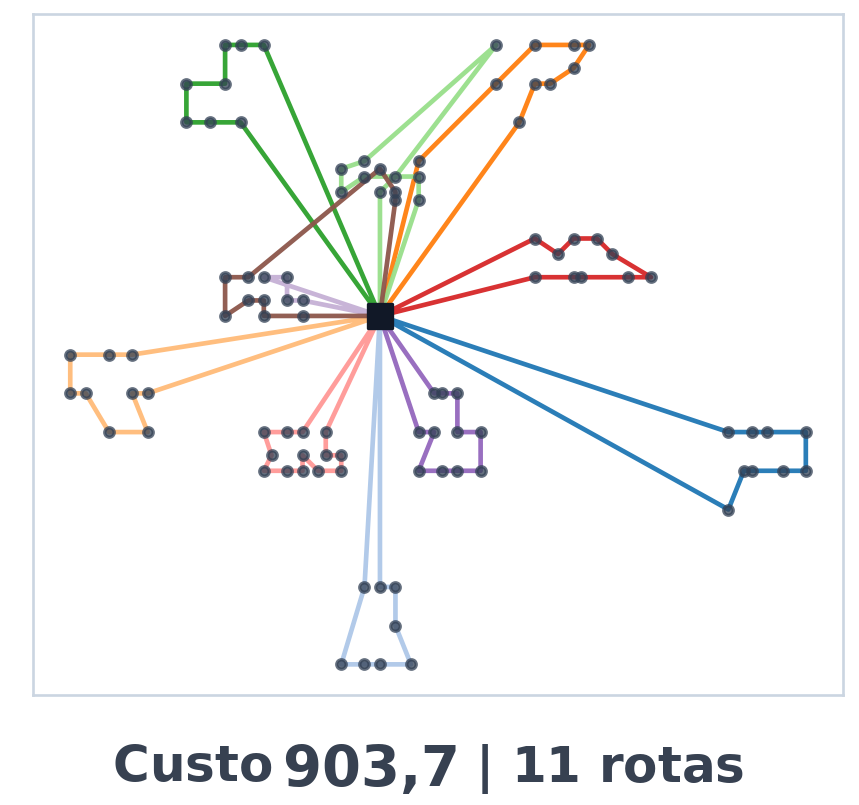
\includegraphics[width=\linewidth]{route_compare_C_panel_2}
        \caption{VND}
    \end{subfigure}
    \hfill
    \begin{subfigure}[t]{0.32\textwidth}
        \centering
        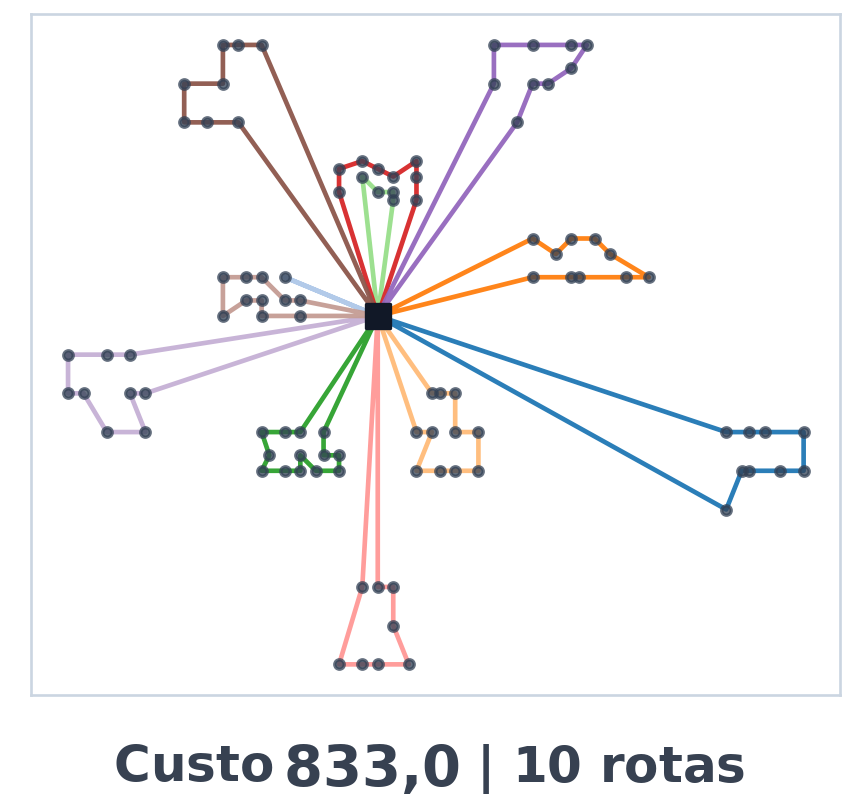
\includegraphics[width=\linewidth]{route_compare_C_panel_3}
        \caption{GRASP fixo}
    \end{subfigure}

    \par\medskip

    \makebox[\textwidth][c]{%
    \begin{subfigure}[t]{0.32\textwidth}
        \centering
        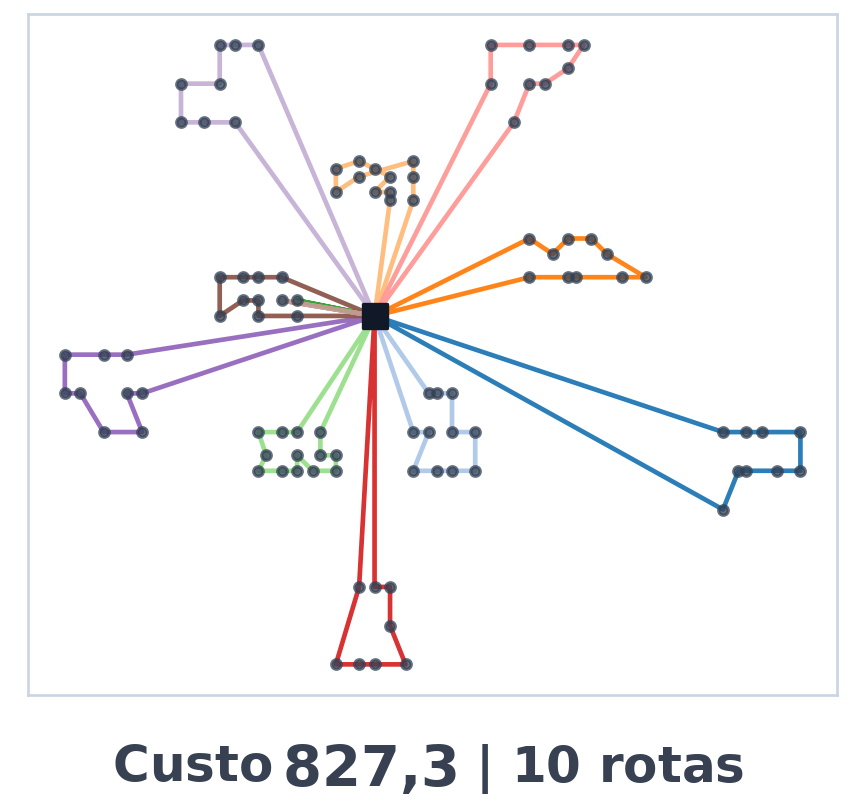
\includegraphics[width=\linewidth]{route_compare_C_panel_4}
        \caption{GRASP reativo}
    \end{subfigure}
    \hspace{0.02\textwidth}
    \begin{subfigure}[t]{0.32\textwidth}
        \centering
        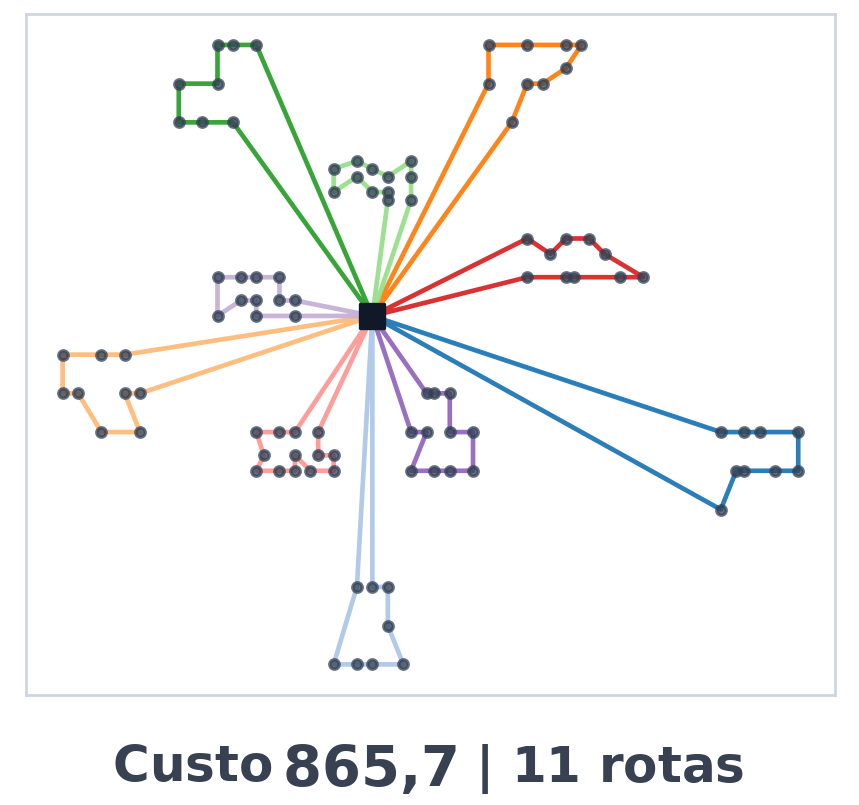
\includegraphics[width=\linewidth]{route_compare_C_panel_5}
        \caption{Busca Tabu}
    \end{subfigure}}
    \vspace{5pt}
    \caption*{Fonte: Produção da própria autora.}
    \caption*{\textit{Descrição da Figura~\ref{fig-rotas}:} figura composta por cinco painéis distribuídos em duas linhas, mostrando as rotas produzidas por diferentes algoritmos na instância C102. Em cada painel, o rodapé informa o custo total e o número de rotas da solução correspondente. O menor custo exibido é 827,3, com 10 rotas, obtido pelo GRASP reativo.}
\end{figure}

Em conjunto, os resultados indicam um ganho de qualidade em relação ao algoritmo construtivo puro e reforçam o potencial da integração entre otimização de rotas e monitoramento por sensores. A próxima etapa concentra-se na finalização dos experimentos computacionais com os algoritmos do solver implementado e na consolidação da integração entre o módulo de sensores e o solver.


% ---------------------------------------------------------------
\section{Atividades Realizadas e Metas Futuras}
\label{sec-atividades}

As Etapas~1, 2 e 3 foram concluídas conforme previsto, abrangendo a revisão bibliográfica, o aprofundamento teórico sobre o algoritmo de Solomon e as tecnologias de sensores, bem como a definição da arquitetura geral do sistema. A Etapa~4 encontra-se parcialmente realizada: uma versão inicial do ambiente de simulação de sensores foi desenvolvida, os algoritmos de roteamento foram implementados e testes iniciais de integração foram conduzidos, permanecendo pendentes a integração completa entre os módulos e a ampliação da validação experimental. A execução parcial da Etapa~4 decorre do fato de que, embora uma versão inicial do ambiente de simulação de sensores tenha sido desenvolvida e testes iniciais tenham sido conduzidos, a integração completa com o processo de replanejamento dinâmico e a validação em maior escala ainda permanecem em andamento. A Etapa~5, correspondente a este relatório parcial, foi concluída.

Para a segunda metade do projeto, as metas concentram-se na consolidação da integração entre sensores e solver, na ampliação dos experimentos comparativos, no desenvolvimento do Digital Twin e da interface de visualização, na realização de testes em cenários mais representativos e na elaboração do Relatório Final.

O Quadro~\ref{qdr-cronograma} apresenta o cronograma de atividades previstas e realizadas. 

\begin{quadro}[H]
	\centering
	\caption{Cronograma de atividades previstas e realizadas do Subprojeto (set./2025 a ago./2026)}
	\label{qdr-cronograma}
	\footnotesize
	\renewcommand{\arraystretch}{2}
	\setlength{\tabcolsep}{3pt}
	\begin{tabular}{| p{5.0cm} *{12}{| c} |}
		\hline
		\rowcolor{lightgray}
		\textbf{Atividade} & \textbf{set.} & \textbf{out.} & \textbf{nov.} & \textbf{dez.} & \textbf{jan.} & \textbf{fev.} & \textbf{mar.} & \textbf{abr.} & \textbf{mai.} & \textbf{jun.} & \textbf{jul.} & \textbf{ago.} \\
		\hline
		Etapa 1 – Estudo dos conceitos básicos, modelagem estatística e revisão bibliográfica sobre otimização de rotas e Digital Twins
		& \totalmente & \totalmente & & & & & & & & & & \\
		\hline
		Etapa 2 – Aprofundamento teórico no algoritmo de Solomon e nas tecnologias de sensores IoT aplicáveis
		& & \totalmente & \totalmente & \totalmente & & & & & & & & \\
		\hline
		Etapa 3 – Proposta de adaptação do algoritmo de Solomon e definição da arquitetura do sistema
		& & & & \totalmente & \totalmente & & & & & & & \\
		\hline
		Etapa 4 – Desenvolvimento dos módulos de simulação, integração de sensores IoT e testes iniciais
		& & & & & \parcialmente & \parcialmente & \parcialmente & & & & & \\
		\hline
		Etapa 5 – Elaboração do Relatório Parcial da Pesquisa
		& & & & & & \parcialmente & \totalmente & & & & & \\
		\hline
		Etapa 6 – Desenvolvimento da plataforma Digital Twin e da interface de visualização de dados
		& & & & & & & & & & & & \\
		\hline
		Etapa 7 – Testes computacionais com o algoritmo e coleta/integração de dados reais
		& & & & & & & & & & & & \\
		\hline
		Etapa 8 – Análise dos resultados, validação do modelo com dados reais e                                                                                                                                                                                                                                                                                                                                                                                                                                                                                                                                                                                                                                                                                                                                                                                                                                                                                                                                                                                                  no sistema
		& & & & & & & & & & & & \\
		\hline
		Etapa 9 – Elaboração do Relatório Final e documentação do projeto
		& & & & & & & & & & & & \\
		\hline
	\end{tabular}
	\vspace{5pt}
	\caption*{Fonte: Produção da própria autora.\\Nota: atividade totalmente realizada (\totalmente), parcialmente realizada (\parcialmente) e não realizada (\naorealizada).}
	\caption*{\textit{Descrição do Quadro~\ref{qdr-cronograma}:} cronograma de 9 etapas ao longo de 12 meses (setembro de 2025 a agosto de 2026), reproduzindo o planejamento original do subprojeto. As Etapas~1 a~3 estão totalmente concluídas; a Etapa~4 encontra-se parcialmente realizada; a Etapa~5 foi concluída; as Etapas~6 a~9 correspondem às metas dos próximos meses.}
\end{quadro}

\renewcommand{\bibsection}{\section*{Referências}}
\begin{thebibliography}{99}

\bibitem[Almeida and Borin(2021)]{de2021plataforma}
ALMEIDA, Lahis G. de; BORIN, Juliana F. Plataforma inteligente e sustentável para coleta de resíduos baseada em IoT e LPWAN. In: WORKSHOP DE COMPUTAÇÃO URBANA (COURB), 2021. \textit{Anais [...]} [S. l.]: SBC, 2021. p. 154--167.

\bibitem[Barth et~al.(2023)]{barth2023data}
BARTH, Linard; SCHWEIGER, Lukas; BENEDECH, Rodolfo; EHRAT, Matthias. From data to value in smart waste management: optimizing solid waste collection with a digital twin-based decision support system. \textit{Decision Analytics Journal}, [S. l.], v. 9, p. 100347, 2023.

\bibitem[Dem\v{s}ar(2006)]{demsar2006statistical}
DEM\v{S}AR, Janez. Statistical comparisons of classifiers over multiple data sets. \textit{Journal of Machine Learning Research}, [S. l.], v. 7, p. 1--30, 2006.

\bibitem[Feo and Resende(1995)]{feo1995greedy}
FEO, Thomas A.; RESENDE, Mauricio G. C. Greedy randomized adaptive search procedures. \textit{Journal of Global Optimization}, [S. l.], v. 6, n. 2, p. 109--133, 1995. DOI: 10.1007/BF01096763.

\bibitem[Glover(1989)]{glover1989tabu}
GLOVER, Fred. Tabu search: part I. \textit{ORSA Journal on Computing}, [S. l.], v. 1, n. 3, p. 190--206, 1989. DOI: 10.1287/ijoc.1.3.190.

\bibitem[Glover(1990)]{glover1990tabu}
GLOVER, Fred. Tabu search: part II. \textit{ORSA Journal on Computing}, [S. l.], v. 2, n. 1, p. 4--32, 1990. DOI: 10.1287/ijoc.2.1.4.

\bibitem[Hansen and Mladenovi\'c(2001)]{hansen2001variable}
HANSEN, Pierre; MLADENOVI\'C, Nenad. Variable neighborhood search: principles and applications. \textit{European Journal of Operational Research}, [S. l.], v. 130, n. 3, p. 449--467, 2001. DOI: 10.1016/S0377-2217(00)00100-4.

\bibitem[L\'opez-Ib\'a\~nez et~al.(2016)]{lopez2016irace}
L\'OPEZ-IB\'A\~NEZ, Manuel; DUBOIS-LACOSTE, J\'er\'emie; C\'ACERES, Leslie P\'erez; BIRATTARI, Mauro; ST\"UTZLE, Thomas. The irace package: iterated racing for automatic algorithm configuration. \textit{Operations Research Perspectives}, [S. l.], v. 3, p. 43--58, 2016. DOI: 10.1016/j.orp.2016.09.002.

\bibitem[Lozano et~al.(2018)]{lozano2018smart}
LOZANO, \'Alvaro; CARIDAD, Javier; DE PAZ, Juan Francisco; VILLARRUBIA GONZALEZ, Gabriel; BAJO, Javier. Smart waste collection system with low consumption LoRaWAN nodes and route optimization. \textit{Sensors}, Basel, v. 18, n. 5, p. 1465, 2018. DOI: 10.3390/s18051465.

\bibitem[Pardini et~al.(2020)]{pardini2020smart}
PARDINI, Kellow; RODRIGUES, Joel J. P. C.; DIALLO, Ousmane; DAS, Ashok Kumar; DE ALBUQUERQUE, Victor Hugo C.; KOZLOV, Sergei A. A smart waste management solution geared towards citizens. \textit{Sensors}, Basel, v. 20, n. 8, p. 2380, 2020. DOI: 10.3390/s20082380.

\bibitem[Potvin and Rousseau(1995)]{potvin1995exchange}
POTVIN, Jean-Yves; ROUSSEAU, Jean-Marc. An exchange heuristic for routeing problems with time windows. \textit{Journal of the Operational Research Society}, [S. l.], v. 46, n. 12, p. 1433--1446, 1995.

\bibitem[Prais and Ribeiro(2000)]{prais2000reactive}
PRAIS, Marcus; RIBEIRO, Celso C. Reactive GRASP: an application to a matrix decomposition problem in TDMA traffic assignment. \textit{INFORMS Journal on Computing}, [S. l.], v. 12, n. 3, p. 164--176, 2000. DOI: 10.1287/ijoc.12.3.164.12636.

\bibitem[Ramson et~al.(2021)]{ramson2021lorawan}
RAMSON, S. R. Jino; VISHNU, S.; KIRUBARAJ, A. Alfred; ANAGNOSTOPOULOS, Theodoros; ABU-MAHFOUZ, Adnan M. A LoRaWAN IoT-enabled trash bin level monitoring system. \textit{IEEE Transactions on Industrial Informatics}, [S. l.], v. 18, n. 2, p. 786--795, 2021.

\bibitem[Resende and Ribeiro(2003)]{resende2003greedy}
RESENDE, Mauricio G. C.; RIBEIRO, Celso C. Greedy randomized adaptive search procedures. In: GLOVER, Fred; KOCHENBERGER, Gary A. (ed.). \textit{Handbook of Metaheuristics}. Boston: Springer, 2003. p. 219--249. DOI: 10.1007/0-306-48056-5\_8.

\bibitem[Toth and Vigo(2002)]{toth2002vehicle}
TOTH, Paolo; VIGO, Daniele (ed.). \textit{The Vehicle Routing Problem}. Philadelphia: SIAM, 2002.

\bibitem[Solomon(1987)]{solomon1987algorithms}
SOLOMON, Marius M. Algorithms for the vehicle routing and scheduling problems with time window constraints. \textit{Operations Research}, [S. l.], v. 35, n. 2, p. 254--265, 1987. DOI: 10.1287/opre.35.2.254.

\end{thebibliography}


\end{document}
